	\documentclass{article}
			
		\usepackage{parskip}
		\usepackage{listings}
		\usepackage{xcolor}
		\usepackage{textcomp}

		%STYLE AND COLOR DEFINITION FOR SOURCE CODE 	
		\newcommand{\PHPamountofcolor}{75}
		\newcommand{\SourceCodeContext}{5}
		%Lets define the php language colors:
		\definecolor{PHP_comment_old}{HTML}{FF8000}
		\colorlet{PHP_comment}{PHP_comment_old!\PHPamountofcolor!black}
		\definecolor{PHP_default_old}{HTML}{000000}
		\colorlet{PHP_default}{PHP_default_old!\PHPamountofcolor!black}
		\definecolor{PHP_keyword_old}{HTML}{6c9c11}
		\colorlet{PHP_keyword}{PHP_keyword_old!\PHPamountofcolor!black}
		\definecolor{PHP_emph1_old}{HTML}{0F58A2}
		\colorlet{PHP_emph1}{PHP_emph1_old!\PHPamountofcolor!black}
		\definecolor{PHP_emph2_old}{HTML}{CCAA00}
		\colorlet{PHP_emph2}{PHP_emph2_old!\PHPamountofcolor!black}
		\definecolor{PHP_emph4_old}{HTML}{C60484}
		\colorlet{PHP_emph4}{PHP_emph4_old!\PHPamountofcolor!black}
		\definecolor{PHP_string_old}{HTML}{C78F0A}
		\colorlet{PHP_string}{PHP_string_old!\PHPamountofcolor!black}
		\definecolor{PHP_variable_old}{HTML}{C82210}%C82210
		\colorlet{PHP_variable}{PHP_variable_old!\PHPamountofcolor!black}
		\definecolor{PHP_number_old}{HTML}{BF1CA6}
		\colorlet{PHP_number}{PHP_number_old!\PHPamountofcolor!black}
		%Now we want to highlight the variables. This will be done by triggering the function \PHPhighlightvar at the start of any $ run. This function wil only highlight variables and any other identifiers will be ignored. Luckily lstlisting will only give correct identifiers so we only will have to check if the previous call was made with a $
		\usepackage{fontspec}
		\setmonofont{Courier}
		%\usepackage[utf8]{inputenc}
		%\usepackage[T1]{fontenc}
		%\usepackage{courier, textcomp}
		\usepackage{etoolbox}
		\newtoggle{InString}{}% Keep track of if we are within a string
		\togglefalse{InString}% Assume not initally in string
		
		\newcommand*{\ColorIfNotInString}[1]{\iftoggle{InString}{#1}{\color{PHP_number}#1}}%

		%helper
		
		\newcommand{\PHPhighlightvar}[1]{\ifnum\theDollarFlag=1 \color{PHP_variable} \fi#1\setcounter{DollarFlag}{0}}
		\newcounter{DollarFlag}
		
		%images
		\usepackage{graphicx}
		\graphicspath{ {images/} }
		\usepackage{wrapfig}
		\usepackage{subcaption}

		
		
			
			
			
		
			
			\title{Artificial Intelligence: \\ Reinforcement Learning project\\ \large Reduced chess end-games }

			\author{Edoardo Ghini}
			
			\begin{document}
			
			\textbf{\maketitle}
			\pagenumbering{gobble}
			
			\bigskip\bigskip\bigskip
			\begin{center}
			
\includegraphics[width=0.5\textwidth]{laSapienza}
			\end{center}
			\bigskip\bigskip\bigskip
			\textbf{
			Dipartimento di Ingegneria dell'Università di Roma La Sapienza}
			

			\newpage
			\pagenumbering{roman}
			\tableofcontents
			\newpage
			\pagenumbering{arabic}
			
			
			
			
			
			%SETTING STYLE OF SOURCE CODE
			\lstset{
		  language        = php,
		  basicstyle      = \footnotesize\ttfamily,
		  keywordstyle    = \color{PHP_keyword},
		  stringstyle     = \color{PHP_string!90!black}\toggletrue{InString},
		  %this allows highlighting of variables:
		  literate        =  {\$}{{\iftoggle{InString}{\$}{\setcounter{DollarFlag}{1}\color{PHP_variable}\$\color{PHP_default}}}}1
		%    {"}{{{\ProcessQuote{"}}}}1% Disable coloring within double quotes
		%    {'}{{{\ProcessQuote{'}}}}1% Disable coloring within single quote
		    {0}{{{\ColorIfNotInString{0}}}}1
		    {1}{{{\ColorIfNotInString{1}}}}1
		    {2}{{{\ColorIfNotInString{2}}}}1
		    {3}{{{\ColorIfNotInString{3}}}}1
		    {4}{{{\ColorIfNotInString{4}}}}1
		    {5}{{{\ColorIfNotInString{5}}}}1
		    {6}{{{\ColorIfNotInString{6}}}}1
		    {7}{{{\ColorIfNotInString{7}}}}1
		    {8}{{{\ColorIfNotInString{8}}}}1
		    {9}{{{\ColorIfNotInString{9}}}}1,
		  identifierstyle = \color{PHP_default}\PHPhighlightvar,
		  commentstyle    = \color{PHP_comment}\slshape,
		  emph            =[1]{require_once, require, include_once, include, namespace, use, class, function, new},
		  emphstyle       =[1]\color{PHP_emph1},%\bf,
		  emph            =[2]{echo, empty, isset, array, instanceof},
		  emphstyle       =[2]\color{PHP_emph2},%\bf,
		  emph            =[3]{var, const, abstract, 
		                        protected, private, public,
		                        static, final, extends, implements,
		                        global, if, else, foreach ,for,
		                        endforeach, endif, endfor, elseif,
		                        as,def},
		  emphstyle       =[3]\color{PHP_keyword},%\bf,
		  emph            =[4]{return, throw, exit, __halt_compiler, continue, break},
		  emphstyle       =[4]\color{PHP_emph4},%\bf,
		  breaklines      = true,
		  captionpos      = b,
		  rulecolor       =\color{black},
		  keywords    ={__halt_compiler,    abstract,   and,    array,
		                    as, break,  callable,   case,   catch,  class,
		                    clone,  const,  continue,   declare,    default,
		                    die,    do, echo,   else,   elseif,
		                    empty,  enddeclare, endfor, endforeach, endif,
		                    endswitch,  endwhile,   eval,   exit,   extends,
		                    final,  finally,    for,    foreach,    function,
		                    global, goto, if,   implements, include,
		                    include_once,   instanceof, insteadof,
		                    interface,  isset, list,    namespace,
		                    new,    or, print, private, protected,  public,
		                    require,    require_once, return,   static,
		                    switch, throw,  trait, try, unset, use, var,
		                    while,  xor,    yield,
		  },
		  numbers=left,
		  stepnumber=1,  
		  numberfirstline=true,
		  numberstyle=\footnotesize,
		  xleftmargin=4.0ex,
		  upquote=true,
		  showlines=true
		  }	
			
			\renewcommand{\lstlistingname}{Code}

			
			\part{Introduction}


			A biologically inspired solution to solve the problem of autonomous learning is reinforcement learning.\medskip\\
			This strategy tries to take advantage of the concept of reward and punishment that is present in nature.\medskip\\
			In fact, it will stimulate an autonomous agent with positive or negative feedbacks after that each action has been accomplished, with the purpose of strengthen the agent's "decision criterion" which brings it to take the best among all the possible actions.\medskip\\
			I have thought that one possible play-ground in which would be possible to experiment a reinforcement learning approach to a problem is, certainly, the widely known game of chess.\medskip\\

\begin{center}	
\begin{figure}
\centering
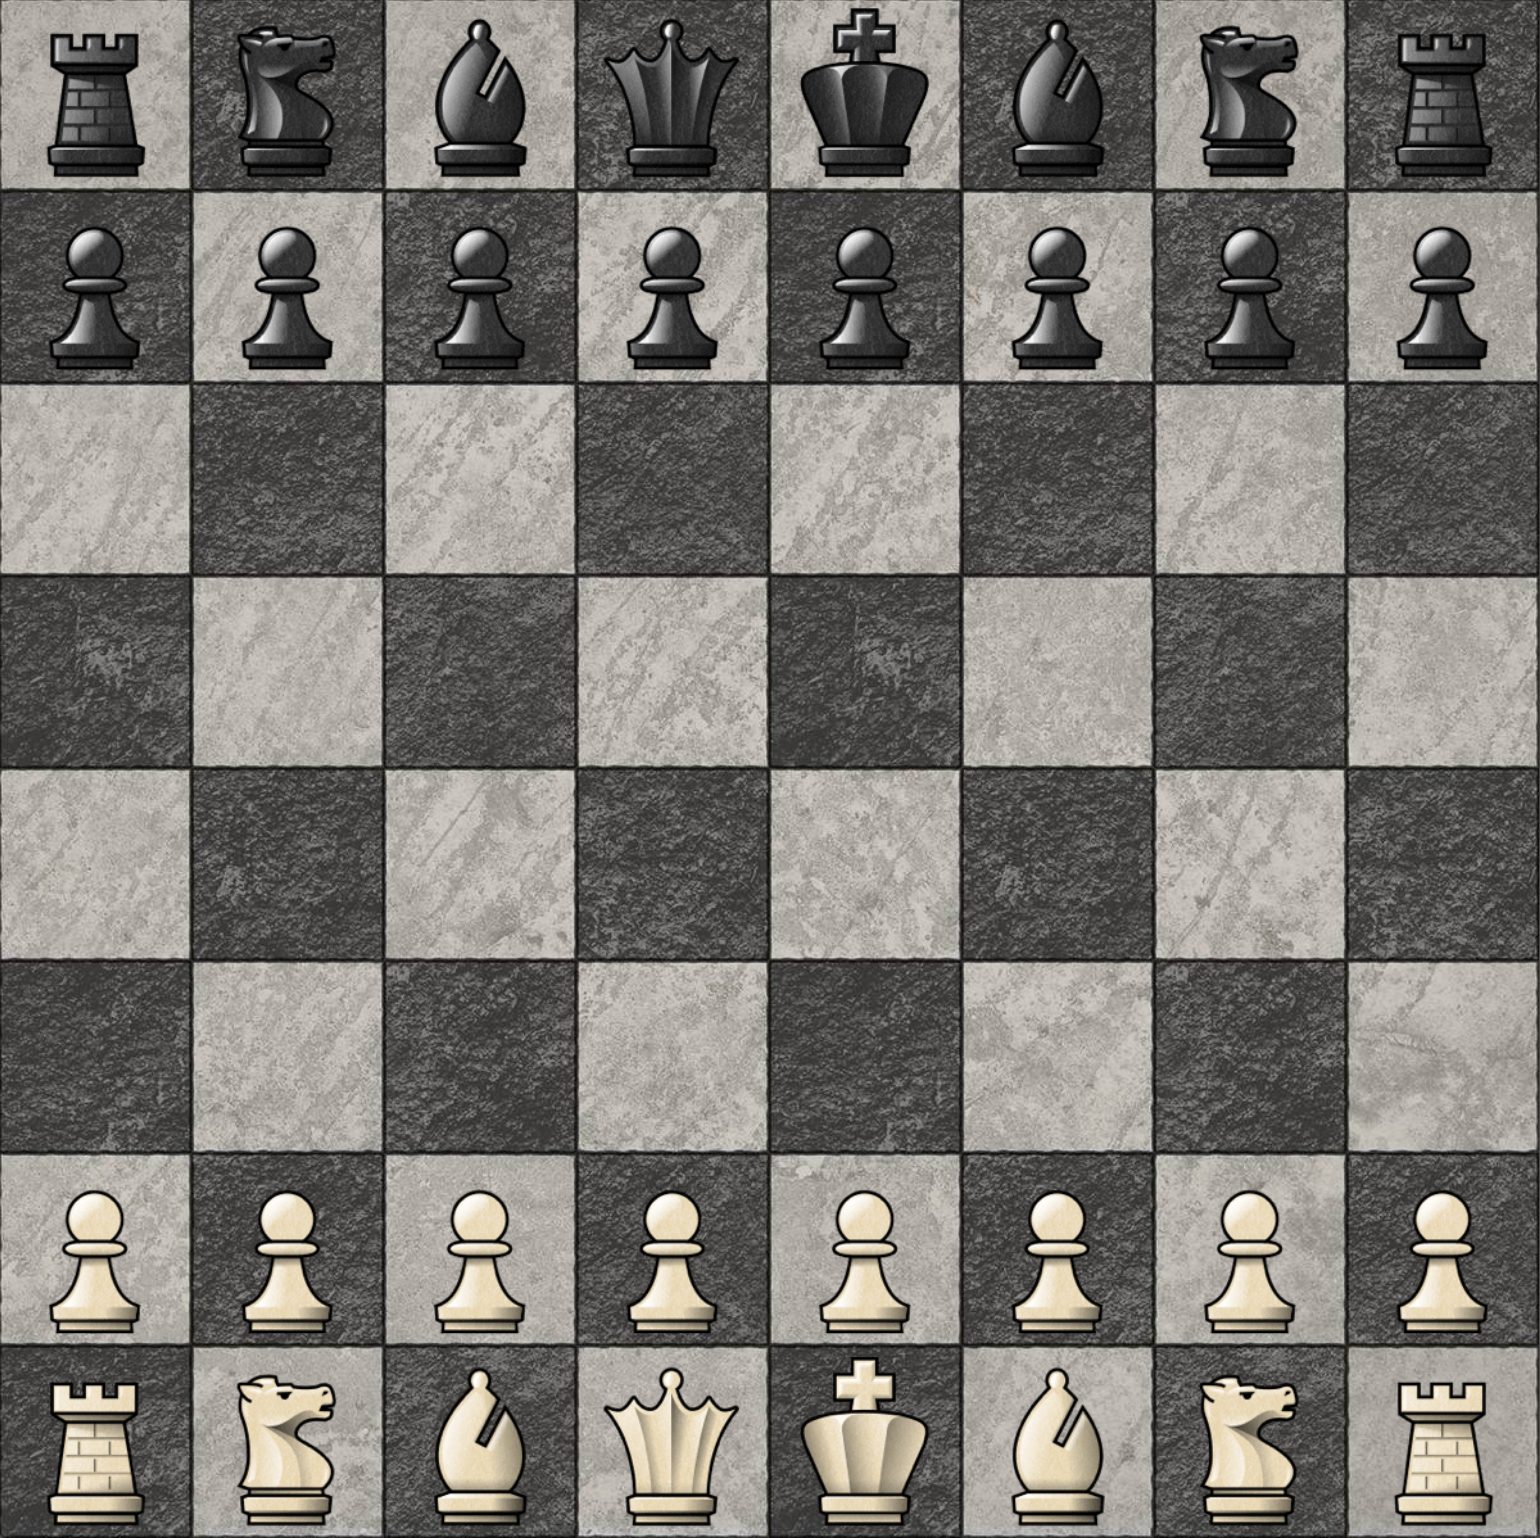
\includegraphics[width=0.5\textwidth]{chess_general}
\caption{the game of chess}
\label{fig:1}
\end{figure}
\end{center}
			

				\newpage
				\part{Development}
				\section{Overview}
				The scenario chosen to develop the project is a chess game in a simplified environment.\medskip\\
				In brief, two agents will play a chess game, one with a random behaviour, the other acting with the objective to maximise the reward given by the environment.\medskip\\
				The autonomous agent, at first, will go through a learning phase using the Every Visit Monte Carlo paradigm.\medskip\\
				Then it will act accordingly to highest expected value contained in the Q-table that was being populated during the learning phase.\medskip\\
				Finally, all the performances will be harvested and arranged in plots that should allow to visualise the effectiveness of the reinforcement learning algorithm.
				\newpage
				\section{Implementative Solution }
				In this section I will describe the general structure of the project in a bottom-up fashion\medskip\\ 
\begin{center}
\begin{figure}[h]
\centering
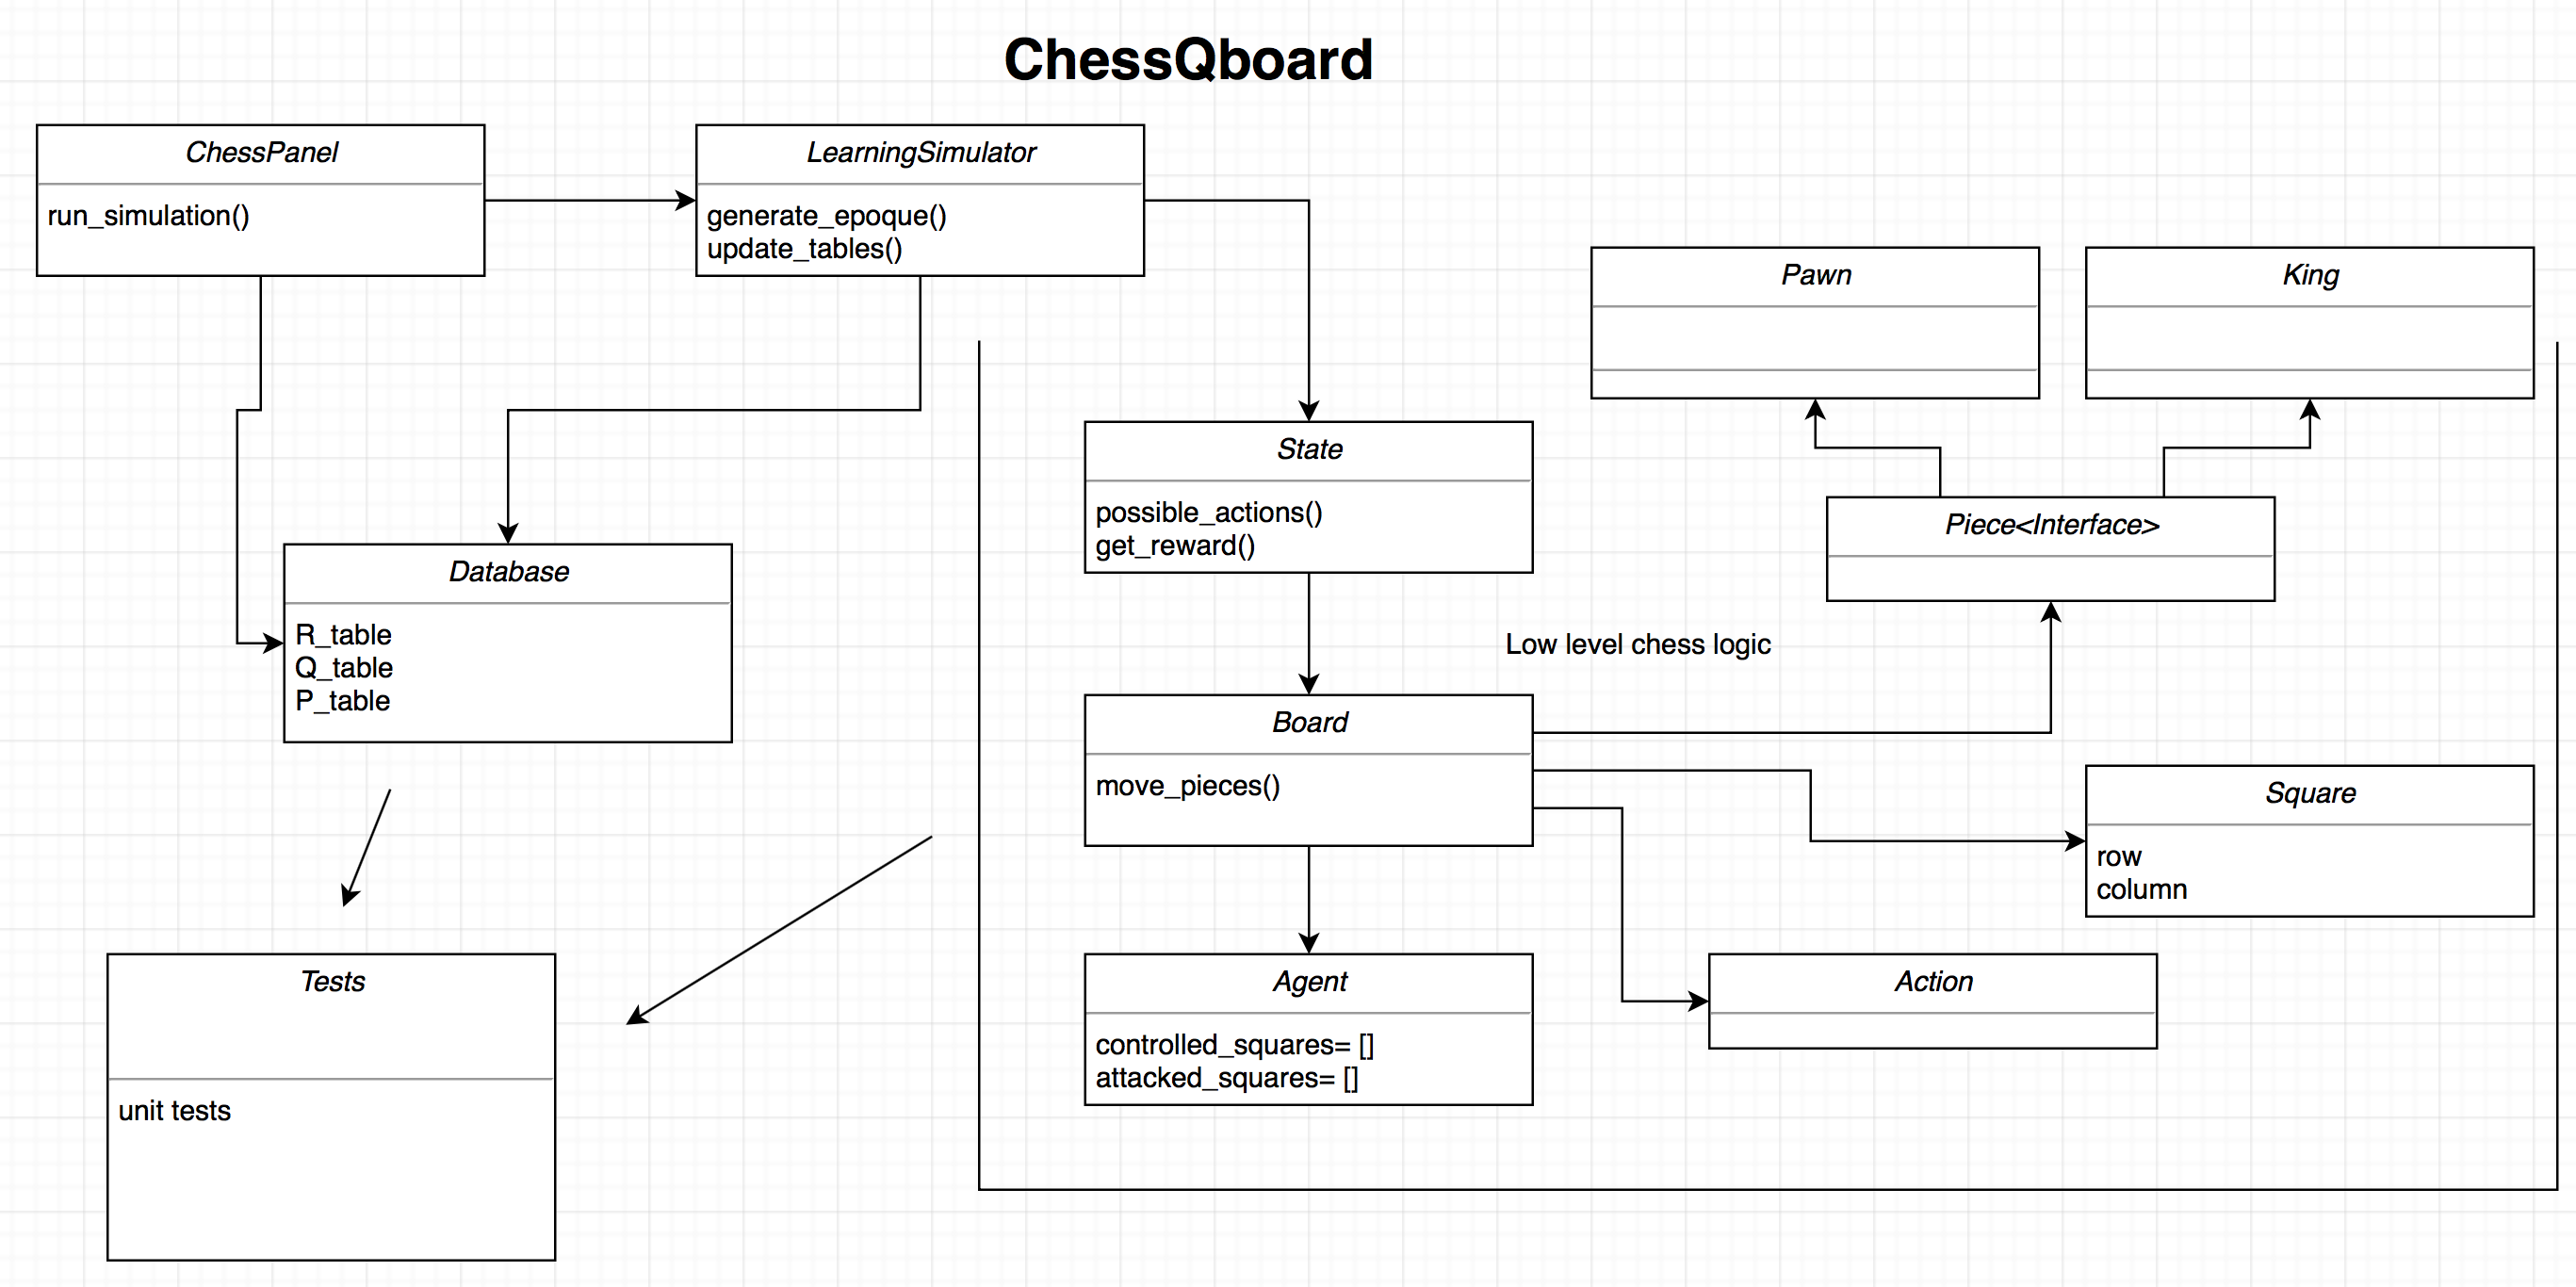
\includegraphics[width=0.99\textwidth]{uml_chess}
\caption{UML scheme of the project}
\label{fig:2}
\end{figure}
\end{center}
				\subsection{Low Level Logic}
				I started from this part of the code, since, implementing the rules and logic of chess would give me a better understanding of the overall problem.\medskip\\
				Python language was chosen because of the great readability of the code. An object oriented paradigm allows to divide the responsibilities of all the low logic to the objects which they belongs.\medskip\\
				All the classes has been created from scratch.\medskip\\
				At first, the wrapper that should act as a bridge between low and high levels is the State class which embodies all the properties of the state of the system, in this case it describes all the chess pieces that are on the chessboard.\medskip\\
				After that, as should be clearer from the UML schema in fig(2), there is a Board class which accomplishes tasks like computing the possible actions at disposal of the agents.\medskip\\
				In order to complete the low level overview there are also Agent, Piece, Square classes among others that helps to carry on high level tasks issued by State class, dividing each in micro tasks.



				\subsection{High Level Logic}
				Starting from the ChessPanel which contains the main calls, the execution flux will go in LearningSim class that probably contains the most meaningful part of the whole implementation.\medskip\\
				In fact, in this class the learning process will be carried out.   The function generate\_epoque will obviously create a series of state action tuples ( a Markov episode) which link the initial state to whatever final state encountered.

				\begin{lstlisting}[caption= generate epoque function, label=exepred]
def generate_epoque(self,iteration_num,epoque_num):
		
	step_number= 0
	state = self.initial_state
	turn= "white"
	state_action_tuples= []
	while step_number <= self.max_epoque_steps and not state.is_final_state_for_agent(turn):
		if turn == "white":
			possible_actions= state.possible_actions("white")
		else:
			possible_actions= state.possible_actions("black")

		#choose an action according to policy with epsilon-greedy and softmax
		action=self.choose_action(state,possible_actions,epoque_num,turn)
		next_state_str= state.execute_action( action )
		
		next_state= State.State(next_state_str)
		sa_tuple= [ state, action, turn]
		state_action_tuples.append( sa_tuple )

		state= next_state
		step_number+=1
		if turn == "white":
			turn= "black"
		else:
			turn= "white"
	if state.is_final_state_for_agent(turn):
		state_action_tuples.append( [state, None, turn ])

	return state_action_tuples
\end{lstlisting}
				\newpage

				\subsection{Monte Carlo Learning Theory}
				For this kind of problems, with huge state spaces that initially are all unknown, it could be convenient to sample some causal "from state, to state"  chains from the state space in uniform way in order to partially explore the search space following a uniformly random distribution ( at least for the first iterations).\medskip\medskip\\These samples are called episodes and are at the base of Monte Carlo algorithm: after that this episodes have been generated, they could be used to update the policy.\medskip\medskip\\
				I opted for a Monte Carlo Q function based update of the policy, instead of the version that uses V function.
				In fact, in retrospect, I think that I used the Q table itself both as concrete representation of the Q function and as the current policy used to decide the best next action. I may be correct in this, since the actual policy gives by definition the action that maximise the current Q function and similarly I choose the action that shows the highest value of expected reward in the actual Q table.\medskip\\
				Finally, I will seek convergence through the update of the aforementioned Q table.

				\newpage
				\subsection{Database Integration}

				At a certain point I had to address the problem of data structure resilience, I wanted to keep in memory three different tables that are necessary for Monte Carlo algorithm and performance tracking.\medskip\\
				Then I opted for usage of a database ( MySql ) that will help also in retrieving some useful informations such the most promising action from a particular state of the chessboard.\medskip\\
				\begin{lstlisting}[caption= db query for best action, label=exepred]
SELECT ACTION FROM QTABLE WHERE STATE="1k1/ppp/111/111/PPP/1K1" AND TURN="white" AND REWARD IN ( SELECT MAX(REWARD) FROM QTABLE WHERE STATE="1k1/ppp/111/111/PPP/1K1" AND TURN="white")
				\end{lstlisting}

				This solution turned to be efficient in terms of data separation and it showed to be extremely to retrieve particular max or average values when they was needed without impacting on the complexity of python code.\medskip\\
				But, on the other hand, it has added a very high time overhead to the code execution since every iteration of the algorithm triggers hundreds of db queries.\medskip\\
				Such a trade off should not be undertaken lightheartedly since the time needed to train the model against a scenario of moderate complexity would skyrocket with the increment of possible states in the agent world.\medskip\\


				\newpage

				\subsubsection{ R and Q tables}
				Among the tables stored in the database there are two that are necessary to the Monte Carlo algorithm execution:\medskip\\
				The R table contains all the actions that have been chosen by agents indexed by a progressive integer and consequently the state from which the agent has done the action, the collected reward and also informations about the current epoque and iteration as shown in fig(3).\medskip\\
		
\begin{center}
\begin{figure}[h]
\centering
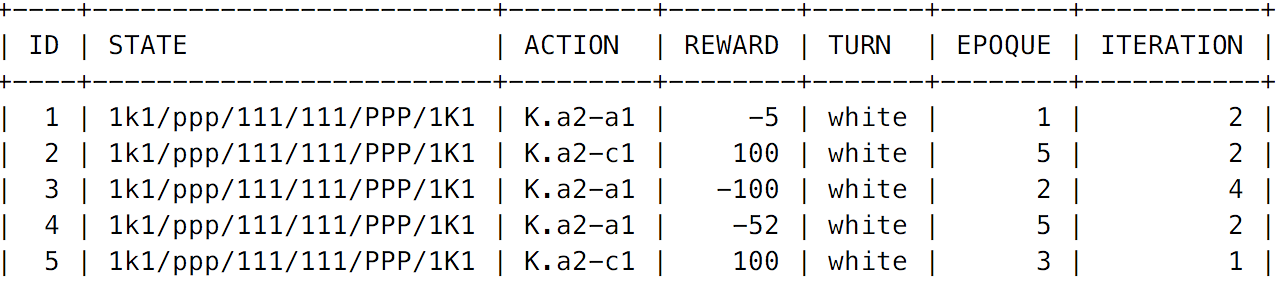
\includegraphics[width=0.9\textwidth]{r_table}
\caption{table of rewards in database}
\label{fig:3}
\end{figure}
\end{center}



				The Q table, in fig(4), instead is composed by a set of state action pairs executed in the past with relative reward. In this data table the unique key is made of state and action attributes that are two strings and they describes uniquely the corresponding python class object in the code.\medskip\\
\begin{center}
\begin{figure}[h]
\centering
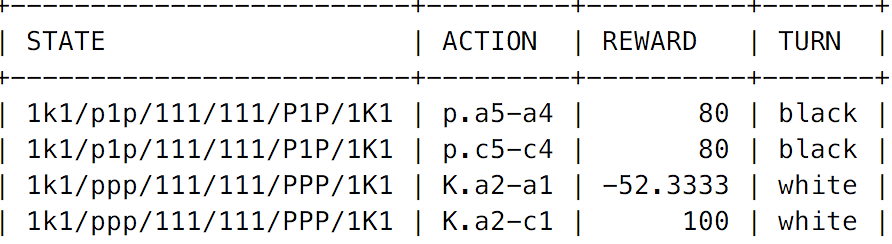
\includegraphics[width=0.9\textwidth]{q_table}
\caption{Q table in database}
\label{fig:4}
\end{figure}
\end{center}
\newpage
				Tanks to this strict correspondence I was able to transfer and memorise strings of states and actions via database and when they where needed in the algorithm execution, they would be parsed and converted in objects.\medskip\\

\begin{lstlisting}[caption=from string to class object, label=exepred]
def parse_action_string( self, action_string, board):
	letters= list(action_string)
	from_square_key = letters[2]+letters[3]
	to_square_key = letters[5]+letters[6]
	self.piece= board.squares[from_square_key].piece
	self.target_square= board.squares[to_square_key]
	self.capture= letters[4] == "x"
	self.check= len(letters) == 8
\end{lstlisting}

				These are examples of the dual nature of the action and of the direct and inverse parsing function.\medskip\\

\begin{lstlisting}[caption=inverse mapping, label=exepred]
def __str__(self):
	if self.capture:
		sign_1= "x"
	else:
		sign_1= "-"

	if self.check :
		sign_2 = "+"
	else:
		sign_2 = ""

	return self.piece.__str__() +"."+ self.piece.square.__str__() + sign_1 + self.target_square.__str__() + sign_2
\end{lstlisting}
				\newpage



				\subsection{Unit Testing}
				Another technique, which I found extremely useful, was to keep bugs in the code under an acceptable level through tests, that will address every single function of the low level logic.\medskip\\

				\subsubsection{Test Suite}
				I grouped every written test in classes specular to the classes which at which they refer.\smallskip\\
				Then, executing them all at once, I was able to fight bug propagation and code regression ( bugs in old code introduced by implementation of new code).\medskip\\
				

				\begin{lstlisting}[caption=one test in State.py, label=exepred]
def test_get_winner(self):
	self.assertEqual( "white", self.final_state_checkmate.get_winner())
	self.assertEqual( "white", self.final_state_pawn_in_last_row.get_winner())
	self.assertEqual( None, self.final_state_stalemate.get_winner())
	self.assertEqual( None, self.drawn_state.get_winner())
	self.assertEqual( None, self.initial_state.get_winner())
\end{lstlisting}
				\subsubsection{TDD}
				Generally, TDD ( Test Driven Development ) could be seen as work backwards, this is due to the fact that first the test of a function would be written, and indeed it will born to fail since the linked function is not implemented yet.\medskip\\
				Then the function would be built with the assurance brought by the test that it will behave as expected.\medskip\\
				I found very reassuring and practical, to develop most of the low level code in this way.\medskip\\
				
				\newpage


				\subsection{Visualising Scenarios}

				There I present some figures which can help to explain what is the problem addressed by the project.\medskip\medskip\\

		\begin{figure}[h]
		\centering
        \begin{subfigure}{0.26\textwidth}
                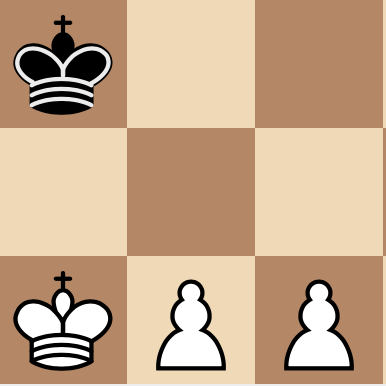
\includegraphics[width=\linewidth]{simple_board}
                \caption{Simple board}
        \end{subfigure}\quad
        \begin{subfigure}{0.26\textwidth}
                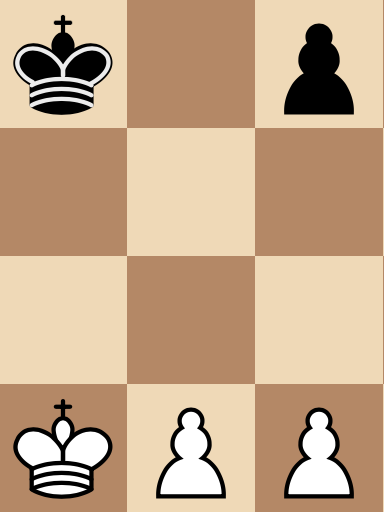
\includegraphics[width=\linewidth]{moderate_board}
                \caption{Moderated Board}
        \end{subfigure}\quad
        \begin{subfigure}{0.26\textwidth}
                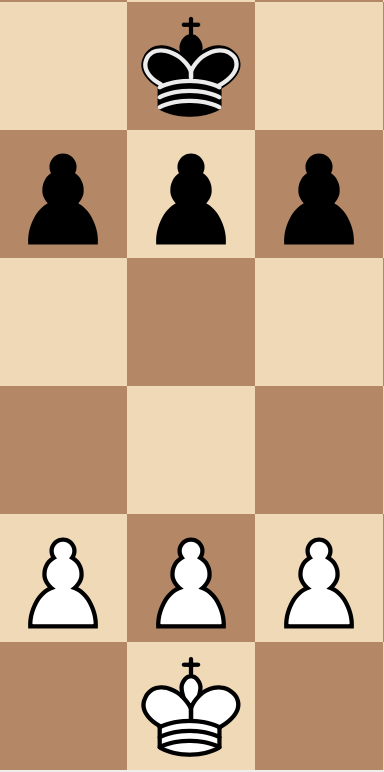
\includegraphics[width=\linewidth]{complex_board}
                \caption{Complex Board}
        \end{subfigure}
 		\label{fig:5}
 		\end{figure}



				Even if the board configurations above seem trivial, there are a lot of possible sequences of states that can be generated from them, therefore this will reduce drastically the chances of convergence.



   				\newpage
             
				
				\section{Results}
				After the learning process has come to an end, the statistics can be drawn from the table of performances that keeps record of the dimension of the Q table, of various averages of rewards and of the winner of the episode for each epoque in each iteration.\medskip\\
				

				\subsection{Displaying an episode}
				Since all the actions undertaken by each agent during episodes have been collected and indexed in the R table of the database, would be possible to display a sort of playback of the chess game.\medskip\\

		\begin{figure}[h!]
		\centering
        \begin{subfigure}{0.23\textwidth}
                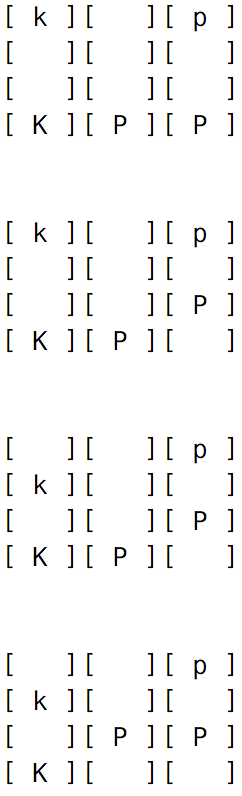
\includegraphics[width=\linewidth]{visual_game_1}
                \caption{1,2,3,4 states}
        \end{subfigure}\qquad
        \begin{subfigure}{0.23\textwidth}
                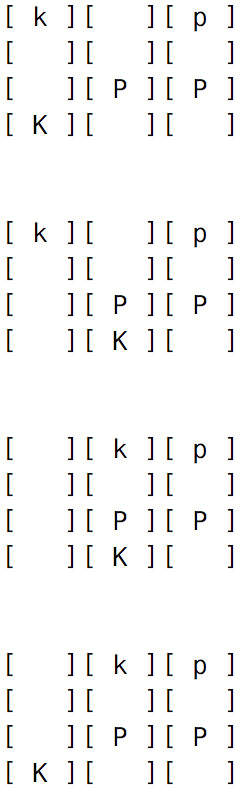
\includegraphics[width=\linewidth]{visual_game_2}
                \caption{5,6,7,8 states}
        \end{subfigure}\qquad
        \begin{subfigure}{0.23\textwidth}
                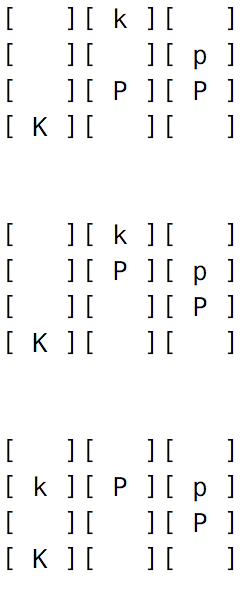
\includegraphics[width=\linewidth]{visual_game_3}
                \caption{9,10,11 states}
        \end{subfigure}
        \caption{Single game execution}
 		\label{fig:6}
 		\end{figure}
				As shown from the images above the state of the board is being modified by agents's actions.\medskip\\


				\subsection{Totally Greedy}
				An interesting possibility would be to exploit to the maximum the estimate of the Q value.\medskip\\\\

				\begin{lstlisting}[caption=greedy run function, label=exepred]
def run_some_greedy_games(self,games_num):
	iteration_num= self.db.get_last_iteration_number()
	iteration_num+=1
	counter=1
	for _ in range(games_num):

		self.simulator= ls.LearningSim(self.initial_board_state ,self.max_epoque_steps,self.agent_chosen,self.db,1,totally_greedy_flag=True)

		winner= self.simulator.montecarlo_epoque_exec(iteration_num,counter)
		self.save_statistics(iteration_num,counter,winner)
		counter+=1
\end{lstlisting}

				\medskip
				This could be achieved by setting the epsilon parameter in a way in which the actions of the autonomous agent will be chosen always with exploitation in mind.\medskip\\
				
				\newpage
				\subsection{P table}

				As I have already mentioned, the P table stores all the statistics of the iterations and from there the performances could be evaluated.\medskip\\
				
\begin{center}	
\begin{figure}[h]
\centering
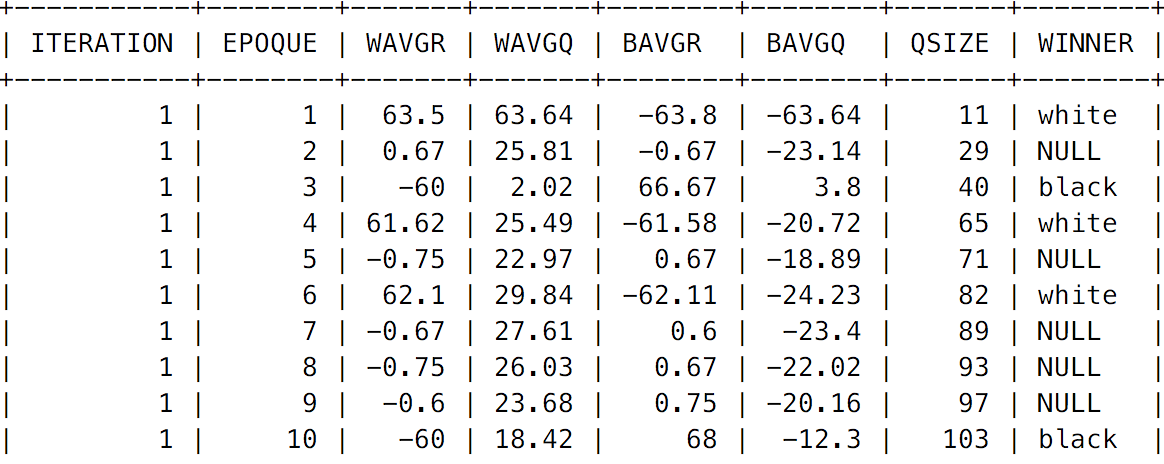
\includegraphics[width=0.9\textwidth]{p_table}
\caption{table of statistics}
\label{fig:7}
\end{figure}
\end{center}

			\subsection{Experiments}
				\subsubsection{Simple Case}
				At the beginning I tried with one of the simplest situations possible as shown in fig. \medskip\\
				With this piece disposition there only the chance to win or stall for the autonomous agent, in other words there are only two possibilities, the learning agent ("white" in this case) wins against the random agent or the game ends by stalemate caused by poor choice of moves of learning agent.\medskip\\
				The depth of the episodes is elementary: two actions at most. In fact the resulting tables after 300 epoques of learning and 30 of greedy playing are very small: 1302 entries in R table and 52 into the Q table.\medskip\\

				\newpage

				\begin{center}	
\begin{figure}[h]
\centering
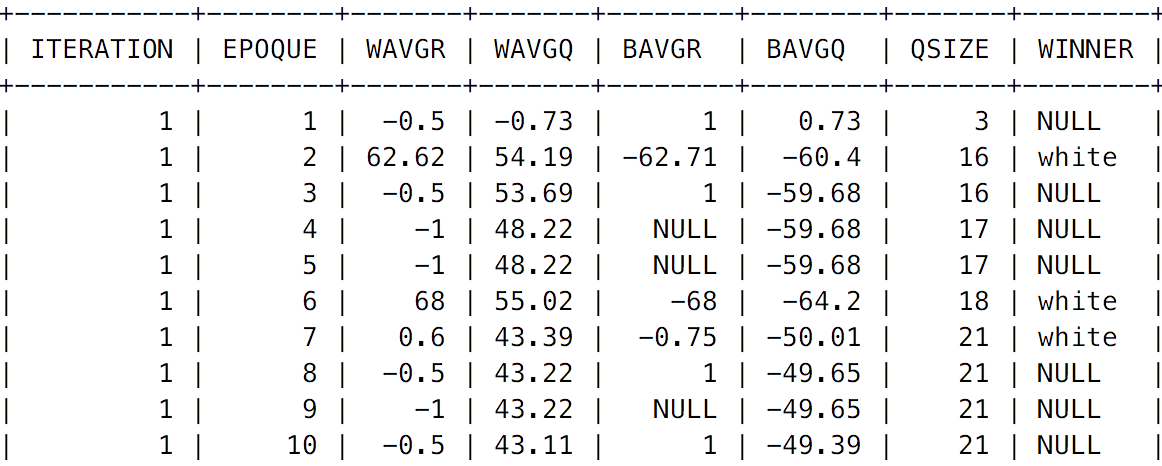
\includegraphics[width=0.9\textwidth]{simple_ptable_ini}
\caption{beginning of the P table}
\label{fig:8}
\end{figure}
\end{center}
\medskip
				From fig(8) is clear how the randomness of action choice due to the epsilon variable the learning agents often makes the wrong choice, however in fig(9) we can see how the agent will perform better in the final stages of learning and during the greedy games: it wins every time.\medskip\\
				\begin{center}	
\begin{figure}[h]
\centering
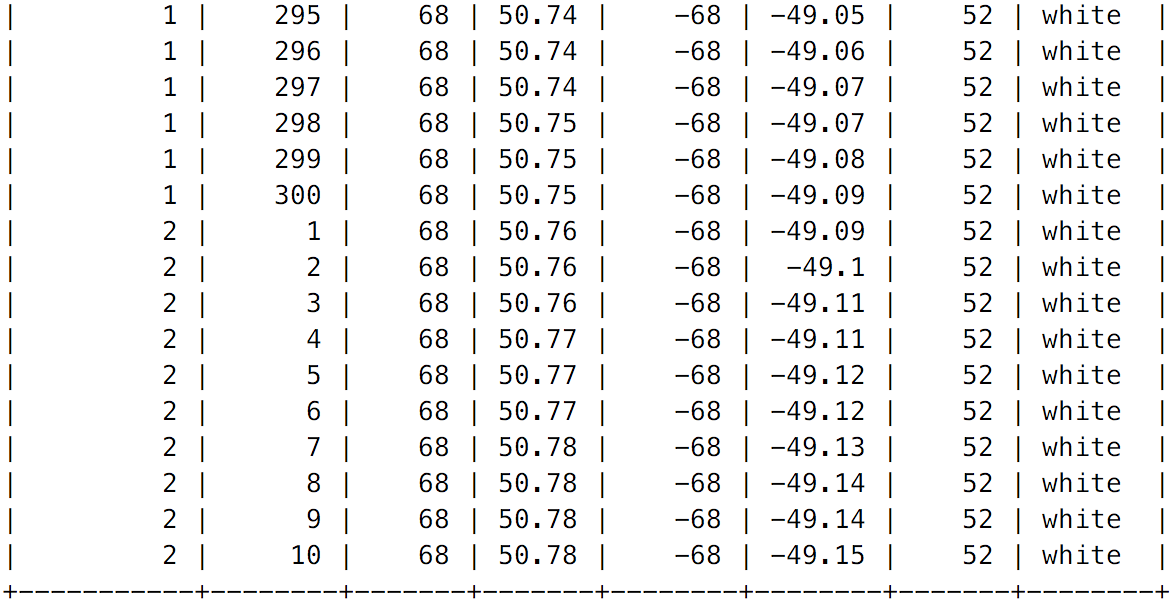
\includegraphics[width=0.9\textwidth]{simple_ptable_fin}
\caption{end of the P table}
\label{fig:9}
\end{figure}
\end{center}

\newpage


				\subsubsection{Moderate Case}
				After the simple case, I tried to solve a slightly more difficult scenario in which the potential outcome of the game was not as mono-directional as in the simple case. This increase of complexity is confirmed by the size of the new tables after the learning phase: this time R table counts 4606 entries and Q table grows up to 1305.
				

\begin{figure}[h!]
		\centering
        \begin{subfigure}{0.50\textwidth}
                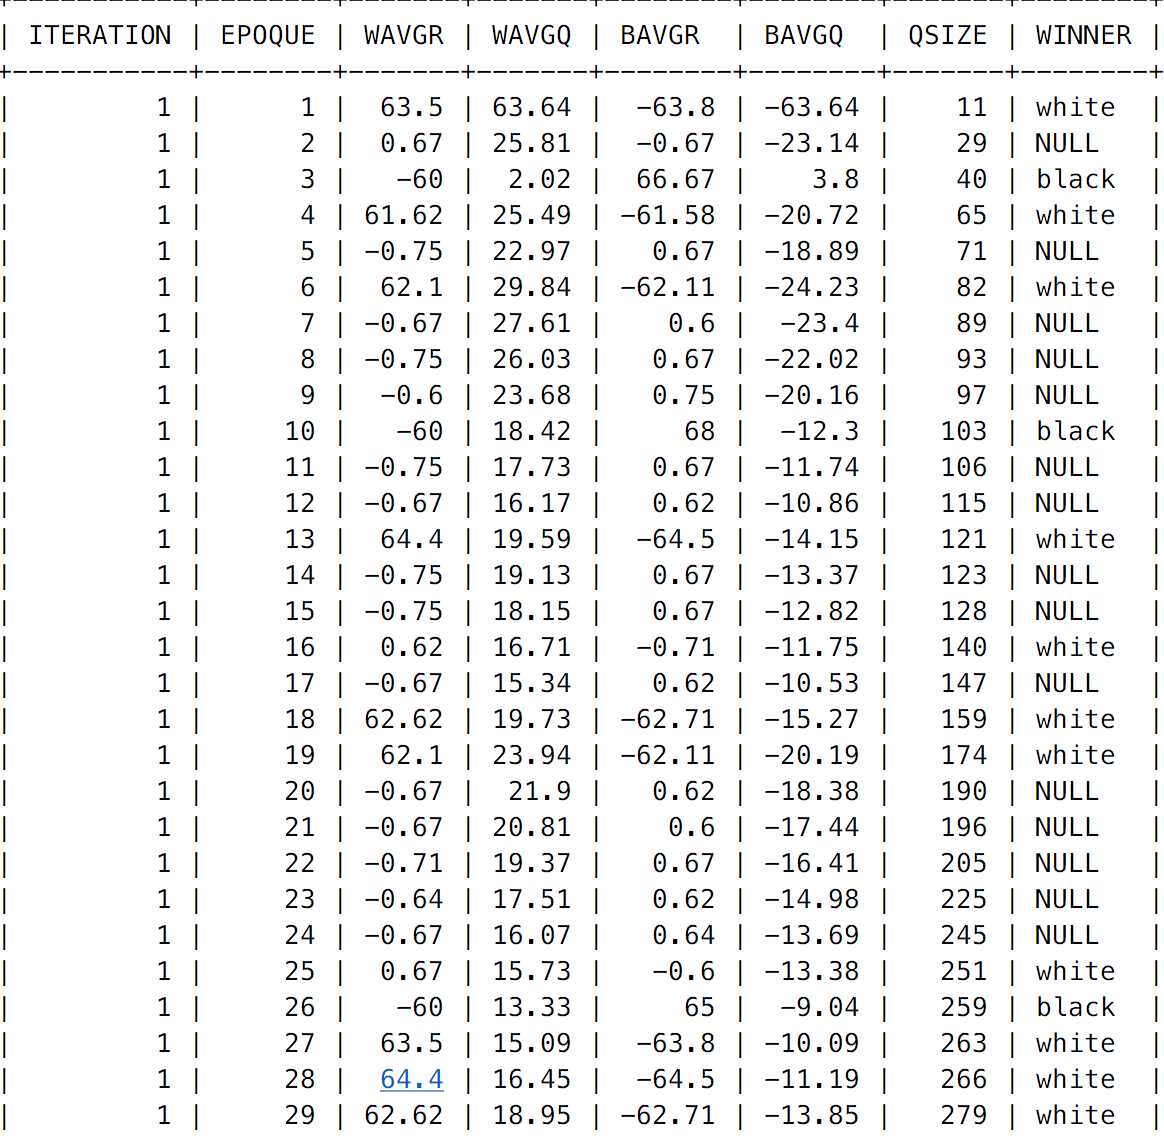
\includegraphics[width=\linewidth]{moderate_ptable_ini}
                \caption{start of P table}
        \end{subfigure}\qquad
        \begin{subfigure}{0.50\textwidth}
                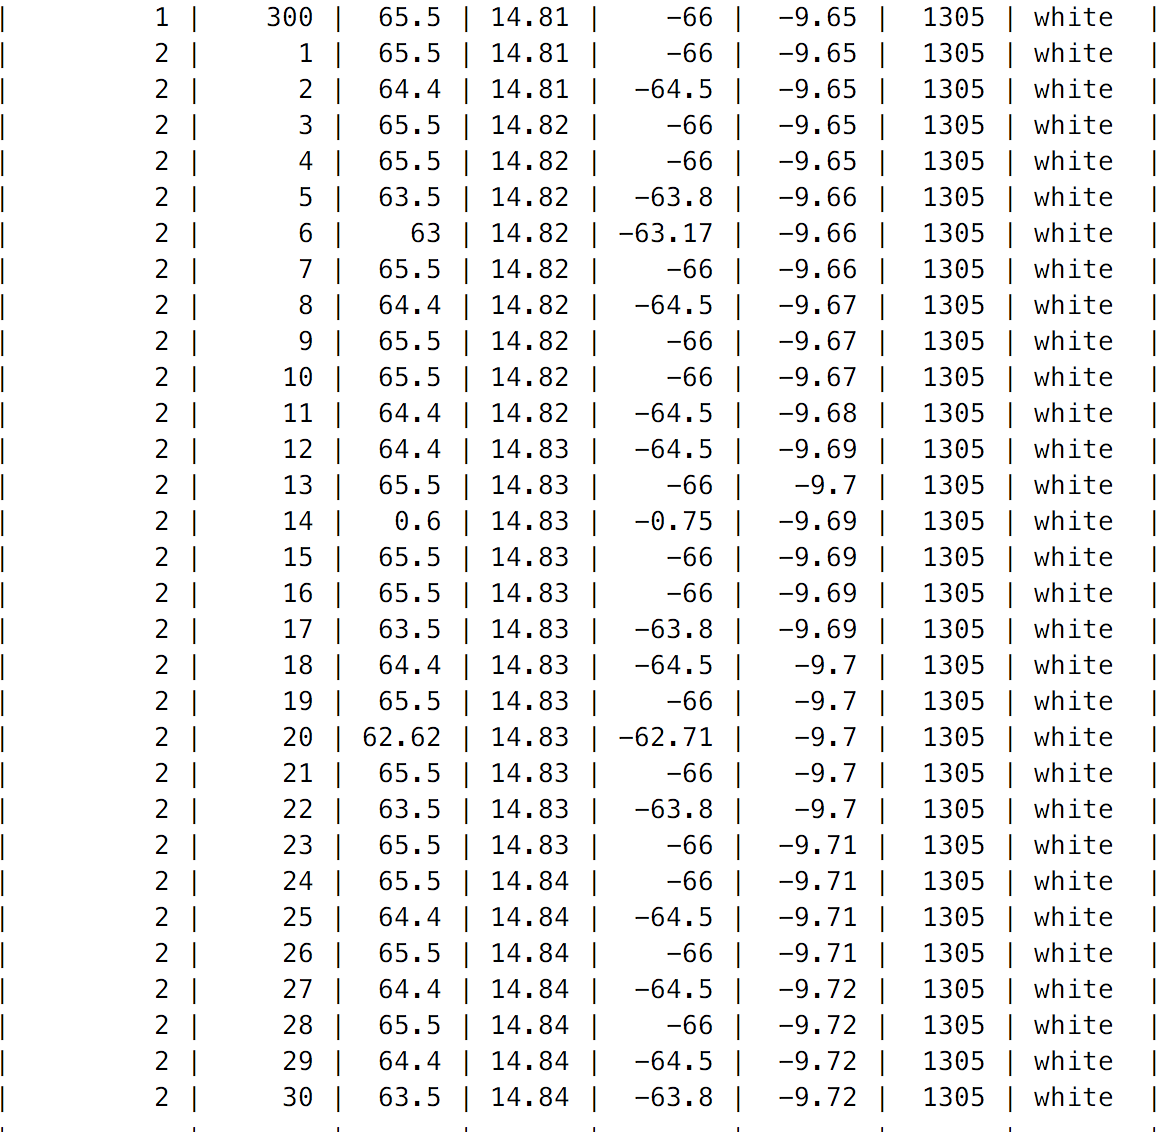
\includegraphics[width=\linewidth]{moderate_ptable_fin}
                \caption{end of P table}
        \end{subfigure}\qquad
        \caption{Performances of moderate case}
 		\label{fig:10}
 		\end{figure}
 		Even if the possible state space is much more extended than the simple case, executing 300 learning epoques and 30 greedy games is sufficient to reach good performances as shown in fig and also the whole process is not very time expensive since it requires at most one minute.


				\subsubsection{Complex Case}
				In the end I tried to work with a complex scenario, obviously this would appear extremely simplified with the respect of the traditional chess board but it is certainly more complicated than simple and moderate cases that I had tried at that time.\medskip\\
				From the starting position is shown in fig(5c), after some attempts of learning iterations with low numbers of epoques, checking the results I thought that the algorithm would require much more learning effort than before.\smallskip\\
				So I began to train the model on 5000 epoques and after that I execute 500 greedy games, the whole process kept going for several hours, almost 20.\smallskip\\

				\begin{figure}[h!]
		\centering
        \begin{subfigure}{0.48\textwidth}
                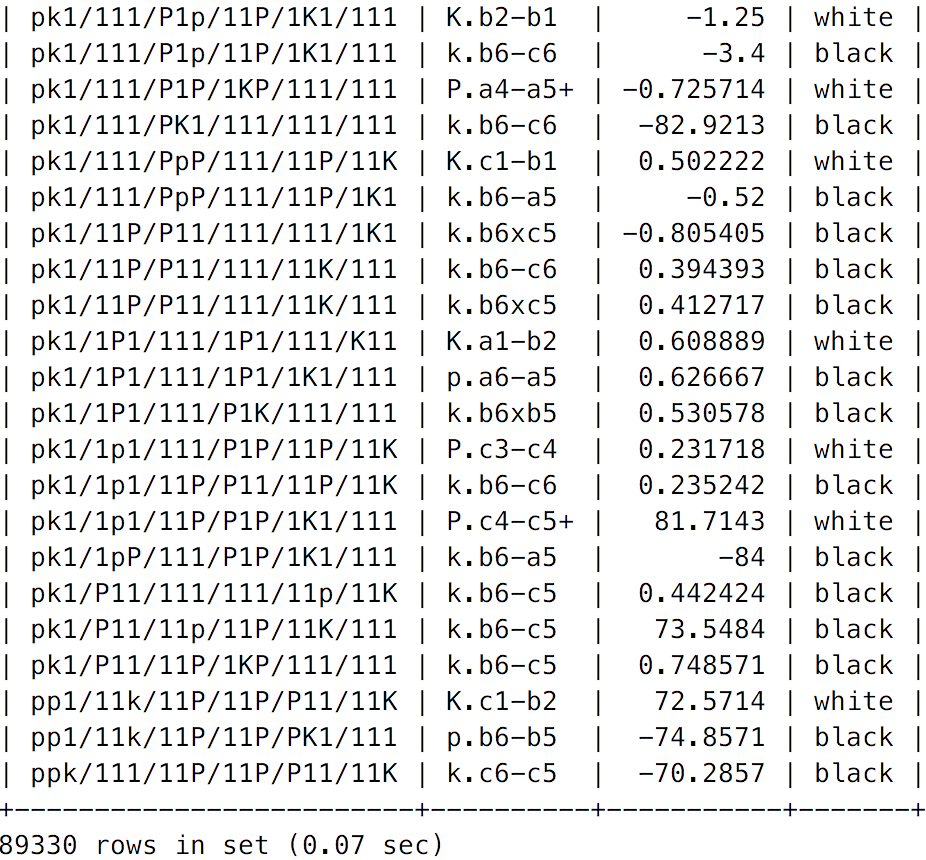
\includegraphics[width=\linewidth]{complex_qtable}
                \caption{Q table}
        \end{subfigure}\qquad
        \begin{subfigure}{0.46\textwidth}
                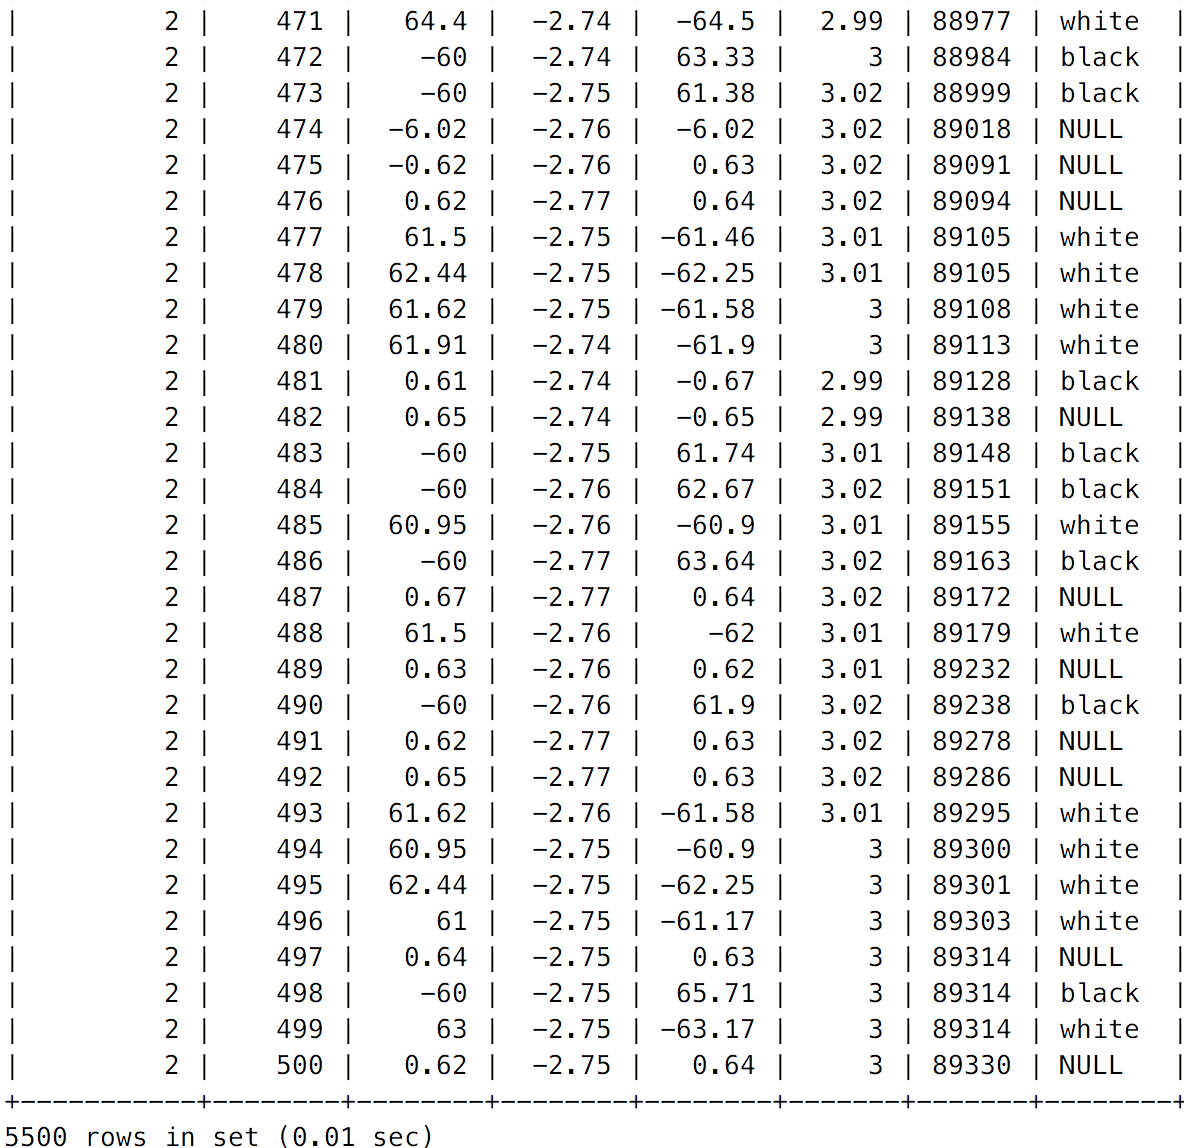
\includegraphics[width=\linewidth]{complex_ptable}
                \caption{P table}
        \end{subfigure}\qquad
        \caption{datatables in complex scenario}
 		\label{fig:11}
 		\end{figure}

				And then I inspect the tables generated which where much larger than the previous experiences:
				as shown in fig(12) R table reached five hundred thousands entries and Q table was just below 90000 entries.\medskip\\
\newpage

				After that, in fig(11b) there is the outcome of the five hundred greedy games.
				In which is clear that the training has given birth to a good policy, even if the difference between games won isn't remarkable.\bigskip
				\begin{center}	
\begin{figure}[h!]
\centering
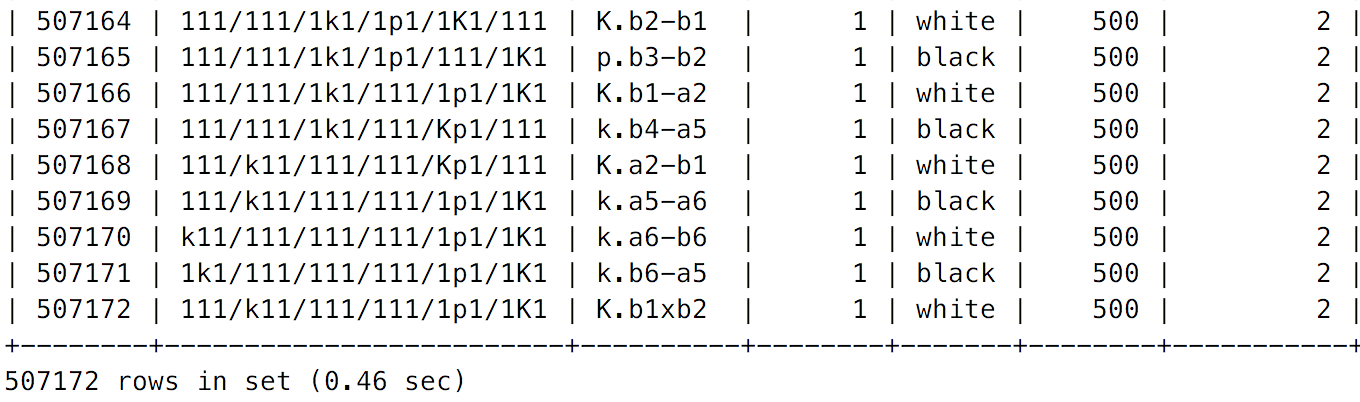
\includegraphics[width=0.9\textwidth]{complex_rtable}
\caption{R table}
\label{fig:12}
\end{figure}
\end{center}


			\section{Conclusions}
			\bigskip\bigskip
			In the final analysis, the model seems to work very well for extremely simple scenarios, but since the state space size increments exponentially with the number of possible actions at disposal of the agent, with more complex experiments also the amount of training computation  needed( and consequently training time ) also grows exponentially.\medskip\\
			The solution concerning the memorisation of data structures should be revised because the introduction of a Database connection causes an unacceptable overhead in terms of time. In fact, observing the computational resources used during learning, turns out that most of the time the python calls to database will wait for long time the response from the DB ( time increases linearly with the size of the tables ).\medskip\\
			This would result in a poor management of the computational capabilities of the cpu which won't go over 30\% of the maximum load and obviously won't even work when the thread is waiting for the DB response.\medskip\\
			On the other hand, with tables stored in secondary memory the learning could be stopped and restarted at will. And, most important, the dynamic table could be accessed from different instances of the DB connection at the same time.\bigskip\\
			This fact hides an implication, there would be the possibility to carry on a distributed learning from different machines that will share the tables in the central Database, this means that every agent at time t will know what all the other agents have learnt until that instant speeding up the convergence.


			
		
				
			
		\end{document}
